\chapter{Prudent Response Surface Models} \label{txt:icarus-chapter}

Machine Learning has rapidly increased in capability and popularity over the past decade \cite{ml-trends-2021, ml-applications-2021}. Today, deep neural networks trained on climate simulation data can produce high-quality predictions at a tiny fraction of the time and computational cost \cite{neural-architecture-search-2021}. In addition, reduced complexity Response Surface Models (RSMs) are adopting newer machine-learning methods \cite{deep-rsm-2020} and are increasingly pushing down the required amount of training data. {\fontfamily{lmss}\selectfont Thus, an idea arises:}

\columnratio{0.4}
\begin{paracol}{2}
    {\fontfamily{lmss}\selectfont
    \begin{center}
        \textit{What if we, too, could train a machine-learning response surface model for our complex process model?}

        \textit{What if it would only take seconds instead of hours to perform a model run?}

        \textit{What if we could use those fast evaluations to run complex Monte Carlo data analysis on our new results?}

        \textit{What if we could do so with even less training data to make retraining cheaper for our frequently evolving complex model?}
    \end{center}

    \noindent Using GPU acceleration, a deep neural network is quickly trained and even performs well on the held-out test dataset. To increase confidence in the results, we add an error bar by having a second network predict the errors of the first. Evaluating this new RSM is fast, and hooking up some data-hungry downstream analysis that consumes the normal distributed predictions is easy.

    \newpar Oh, how soaring our celebration of success! Just before applying the RSM to input data from around the world, we check the input feature distribution. One of the features was constant during training. Changing it to any other value has absolutely no impact on the error bar. Validating the RSM on more testing data reveals that the predicted error bars are in no relation to the growing prediction error. Our confidence sinks.
    }

    \switchcolumn

    \begin{figure}[H]
        \centering
        
\includegraphics[width=0.55\textwidth]{icarus/figures/icarus.png}
        \caption[Icarus Fallen by C\'elestin Nanteuil]{Icarus Fallen (1845) by C\'elestin Nanteuil \cite{icarus-1845}. The New York Public Library. Available in the public domain.}
    \end{figure}
\end{paracol}

{\fontfamily{lmss}\selectfont
\newpar \textit{What if the seemingly simple downstream data analysis performed on the RSM's predictions also queried the RSM on similarly novel inputs? What if the RSM made gross mispredictions for those inputs, too, without any warning that it had been driven beyond its limits? How could we trust the final results of this analysis?}

\newpar Freefall. Daedalus weeps.
}

\section{The Virtue of Prudence} \label{txt:prudent-rsm}

Performing scientific analysis depends on knowing the uncertainty around a measurement or simulation result and assigning varying levels of confidence to a conclusion. As the quality of machine learning methods increases, it may be tempting to use a well-performing model and take its predictions at face value. However, prediction models make mistakes. \Cref{txt:uncertainty-quantification} has reviewed several methods that can be used to estimate the error that a prediction model might make, i.e. to quantify its uncertainty. However, models can also be fed with out-of-distribution inputs that differ vastly in their structure from what the model was trained on, which \Cref{txt:novelty-detection} has discussed. For example, suppose a model trained to predict a cat's age is presented with a picture of the Andromeda galaxy. In that case, neither the predicted age nor the estimated uncertainty likely makes much sense. Therefore, a machine-learning model should be \textit{prudent} in such cases.

\newpar We define being \textbf{prudent} as ``showing good judgment in avoiding risks and uncertainties'' \cite{prudent-dictionary-2023}, following the Cambridge Academic Content Dictionary. In the context of machine-learning-based response surface models (RSMs), a prudent RSM should:
\begin{enumerate}
    \item communicate how \textbf{confident} the RSM is that it can make a prediction at all
    \item communicate the level of \textbf{uncertainty} in its prediction
    \item exercise \textbf{prudence} by avoiding overconfident predictions
\end{enumerate}
\noindent In this chapter, we present the Icarus architecture for prudent RSMs (\Cref{txt:icarus-rsm}) and highlight how its predictions, uncertainty, and confidence can be utilised (\Cref{txt:icarus-propagation}). The components of this architecture are explored individually in \Cref{txt:ood-detection-chapter}, \Cref{txt:prediction-chapter}, and \Cref{txt:uncertainty-chapter} using a new dataset introduced in \Cref{txt:sosaa-data-chapter}. In \Cref{txt:icarus-evaluation-chapter}, we put Icarus to the test and build and evaluate an RSM for the SOSAA model (see \Cref{txt:sosaa-model}). Finally, \Cref{txt:icarus-preview} closes with some conclusions and a more detailed preview of the following chapters.

\section{Icarus: An Architecture for Prudent Response Surface Models} \label{txt:icarus-rsm}

The \textbf{Icarus} architecture combines three modules to construct \textit{prudent} response surface models (RSMs, see \Cref{txt:response-surface-models}). The architecture does not specify how these modules should be implemented but provides a blueprint for combining them. The most well-known component of Icarus is its \textcolor{icarus-prediction}{\textbf{prediction model}}, which is tasked with predicting the target variable $Y$ for new inputs $X$ to approximate the response surface of the underlying process that the RSM is being fitted to. The prediction model is trained with pairs of inputs $x \in X_{\text{train}}$ and their corresponding outputs $y$. These input-output pairs come from a set of training data, which represents the in-distribution. It is important to note that existing response surface models have primarily performed only this prediction task and can be used as a prediction model inside Icarus. In other words, an existing RSM can be wrapped with the Icarus architecture to extend its functionality and make it prudent.

The prediction model only produces point-predictions \textcolor{icarus-prediction}{$\hat{Y}$}. However, the prediction target variable $Y$ may have intrinsic aleatoric uncertainty, meaning some inputs may not correspond to just one true value but rather a distribution of values. Furthermore, the prediction model is generally imperfect and may thus predict values that are close but not equivalent to any true value. Therefore, the second component of Icarus is an \textcolor{icarus-uncertainty}{\textbf{uncertainty quantifier}} that is tasked with quantifying the prediction uncertainty of the prediction model. Given the input $X$ and point-prediction \textcolor{icarus-prediction}{$\hat{Y}$}, it estimates the distribution of true values $Y$ around the prediction \textcolor{icarus-prediction}{$\hat{Y}$}, which allows separating aleatoric uncertainty in the data from epistemic uncertainty in the prediction model (see \Cref{txt:aleatoic-epistemic-uncertainty}). We denote this uncertainty distribution with \textcolor{icarus-uncertainty}{$\hat{\Sigma}$}. Since prediction models usually perform worse outside their training data, the uncertainty quantifier should be trained and calibrated on a validation data set that is disjoint from the predictor training data but also comes from the in-distribution.

It is worth remembering that both the prediction model and uncertainty quantifier are only trained on in-distribution training data and can thus only perform their tasks on unseen inputs that are also in-distribution. To avoid trusting their predictions for out-of-distribution (OOD) inputs, the third and most crucial component of the Icarus architecture is an \textcolor{icarus-confidence}{\textbf{out-of-distribution detector}}. Given an unseen input $x \in X$, it is tasked with identifying whether $x$ is in-distribution, i.e. comes from the same distribution as the training data. The OOD detector produces a confidence score \textcolor{icarus-confidence}{$c$} between zero and one that represents the probability that the input comes from the in-distribution and that the prediction model and uncertainty quantifier can produce valid estimates. In the most general case, only the in-distribution (ID) training dataset is available and has to suffice for training the OOD detector. However, by identifying an existing dataset as out-of-distribution or synthesising OOD inputs, the OOD detector can also be trained and calibrated with both ID and OOD inputs.

\begin{figure}[H]
    \centering
    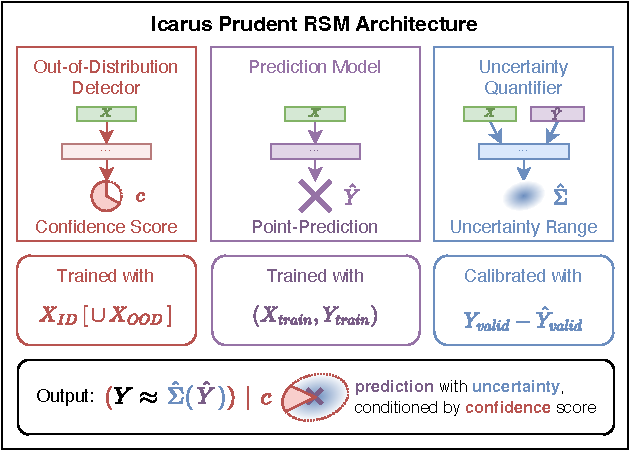
\includegraphics[width=0.915\textwidth]{icarus/figures/icarus-rsm.pdf}
    \caption[Overview of the prudent Icarus RSM Architecture]{Overview of the prudent Icarus RSM Architecture, which consists of three components. The out-of-distribution detector predicts a confidence score \textcolor{icarus-confidence}{$c$}, the prediction model estimates the target variable $Y$ with a point-prediction \textcolor{icarus-prediction}{$\hat{Y}$}, and the uncertainty quantifier predicts and calibrates the prediction uncertainty distribution \textcolor{icarus-uncertainty}{$\hat{\Sigma}$}. Inspired by \textcite{learning-ood-confidence-2018}, the uncertain output prediction is conditioned on the confidence score.}
    \label{fig:icarus-rsm}
\end{figure}

\noindent \Cref{fig:icarus-rsm} provides an overview of the architecture of the Icarus RSM and its three components described above. Crucially, the Icarus RSM does not only report a point-prediction \textcolor{icarus-prediction}{$\hat{Y}$}, but outputs a prediction with its uncertainty \textcolor{icarus-uncertainty}{$\hat{\Sigma}$}. Moreover, both the prediction and the uncertainty are conditioned on an additional output, the confidence score \textcolor{icarus-confidence}{$c$}. Thus, the output of an RSM following the Icarus architecture can be interpreted as follows:

\newpar For any input in $X$, the RSM predicts an output $\textcolor{icarus-confidence}{(}Y \sim \textcolor{icarus-uncertainty}{\hat{\Sigma}(}\textcolor{icarus-prediction}{\hat{Y}}\textcolor{icarus-uncertainty}{)}\textcolor{icarus-confidence}{) \given c}$. For the given confidence level \textcolor{icarus-confidence}{$c$}, the input is out-of-distribution with probability $1-\textcolor{icarus-confidence}{c}$, and the RSM's prediction $\textcolor{icarus-uncertainty}{\hat{\Sigma}(}\textcolor{icarus-prediction}{\hat{Y}}\textcolor{icarus-uncertainty}{)}$ must be ignored. With probability \textcolor{icarus-confidence}{$c$}, the input is in-distribution, and a valid prediction has been made. In this case, the RSM predicts that the true output $Y$ is drawn from the distribution $\textcolor{icarus-uncertainty}{\hat{\Sigma}(}\textcolor{icarus-prediction}{\hat{Y}}\textcolor{icarus-uncertainty}{)}$, which describes the uncertainty in the point-prediction \textcolor{icarus-prediction}{$\hat{Y}$}. While the uncertainty distribution is typically assumed to be normal, i.e. $Y \sim \text{N}(\textcolor{icarus-prediction}{\hat{Y}}, \textcolor{icarus-uncertainty}{\sigma^2(}\textcolor{icarus-prediction}{\hat{Y}}\textcolor{icarus-uncertainty}{)})$ or more concisely $Y \approx \textcolor{icarus-prediction}{\hat{Y}} \textcolor{icarus-uncertainty}{\pm \sigma}$, the more general notation of $Y \sim \textcolor{icarus-uncertainty}{\hat{\Sigma}(}\textcolor{icarus-prediction}{\hat{Y}}\textcolor{icarus-uncertainty}{)}$ also allows for non-normal uncertainty distributions.

\section{Propagating Confidence and Uncertainty} \label{txt:icarus-propagation}

A response surface model built with the Icarus architecture predicts confidence and uncertainty alongside the target value prediction. With the interpretation given above, RSM predictions on out-of-distribution inputs, inputs with high aleatoric or epistemic uncertainty, and inputs with an accurately predicted single true value can all be used and analysed together. If we want to perform some downstream analysis on these predictions, it is crucial to propagate both confidence and uncertainty through all analyses to the final result. In this section, we briefly outline several possible approaches for this propagation.

\newpar Monte Carlo analysis provides an intuitive, easy-to-implement approach for propagating confidence and uncertainty. Here, each prediction is interpreted as a random variable:
\begin{equation*}
    \textcolor{icarus-confidence}{(}Y \sim \textcolor{icarus-uncertainty}{\hat{\Sigma}(}\textcolor{icarus-prediction}{\hat{Y}}\textcolor{icarus-uncertainty}{)}\textcolor{icarus-confidence}{) \given c} = \begin{cases}
        \textcolor{icarus-confidence}{\text{OOD}} &\quad \text{with probability } 1-\textcolor{icarus-confidence}{c} \\
        Y \sim \textcolor{icarus-uncertainty}{\hat{\Sigma}(}\textcolor{icarus-prediction}{\hat{Y}}\textcolor{icarus-uncertainty}{)} &\quad \text{otherwise}
    \end{cases}
\end{equation*}
where the uncertainty distribution $\textcolor{icarus-uncertainty}{\hat{\Sigma}(}\textcolor{icarus-prediction}{\hat{Y}}\textcolor{icarus-uncertainty}{)}$ is sampled with probability \textcolor{icarus-confidence}{$c$}. Otherwise, the result is an \textcolor{icarus-confidence}{OOD} sentinel value that poisons the calculation, similar to \texttt{None}, \texttt{null}, or \texttt{NaN} values that cannot be used in further calculations. All prediction random-variables are sampled repeatedly, and the analysis is performed for each such sample. Clearly, analysis cannot be performed on poisonous OOD sentinel values. Therefore, the analysis is only performed on the ID samples, and the fraction of successful analyses is carried through as the confidence value of the analysis result. Finally, the distribution of all analysis results can be interpreted again as having a confidence value and an uncertainty distribution around a point-prediction value, e.g. the mean of the distribution.

\newpar The propagation of confidence can be seen as a monadic computation. For analyses that combine data points independently, e.g. when calculating the mean squared error over several predictions, the average confidence is propagated to the output. For analyses that analyse pairs of data points, the product confidence $\textcolor{icarus-confidence}{c_1} \cdot \textcolor{icarus-confidence}{c_2}$ is propagated. Both of these cases are intuitively handled with Monte Carlo analysis but can also be calculated analytically. Is this also possible for uncertainty propagation?

\textcite{correlated-propagation-2016} has introduced the \texttt{Measurements.jl} Julia package that uses linear error propagation theory to propagate the uncertainties of independent normally distributed measurements through analysis code in Julia. Specifically, a measurement variable \texttt{x} can be constructed as a mean value and standard deviation using the intuitive \texttt{x = 8.4 $\pm$ 0.7} syntax. Since the measurement type is a subtype of Julia's \texttt{AbstractFloat} abstract type, it can be used directly inside most numerical calculations and algorithms. For instance, \texttt{x+2} evaluates to \texttt{10.4 $\pm$ 0.4} and \texttt{2x} to \texttt{16.8 $\pm$ 1.4}. To handle the creation of correlated uncertainties, e.g. \texttt{x - x}, the measurement type internally keeps track of all independent measurements it is made up of, together with their associated uncertainties, an idea borrowed from the \texttt{uncertainties} Python package with similar functionality \cite{uncertainties-python-2022}. What if the input measurements have non-normally distributed uncertainties or are correlated? \textcite{srsm-phd-1999} presented methods to decompose uncertainties into independent (standard) normal random variables in their work on Stochastic RSMs (see \Cref{txt:stochastic-rsm}), which can be applied here as well. Uncertainties can be handled analytically without manual computation from the user using these approaches.

However, using subclassing and operator overloading can come with extraneous runtime overhead, especially for dynamically tracking all correlations, even though not all may be needed for the final result. As \textcite{autodiff-applications-2021} notes, auto-differentiation (see \Cref{txt:auto-differentiation}) can be generalised beyond automatically generating the code for derivative calculations to also be applied to automatically propagate uncertainties. While subclassing is one possible implementation of auto-differentiation, tools such as Tapenade \cite{tapenade-autodiff-2013} can be applied directly to source code and transform it to compute the derivatives alongside the values. A similar approach could be taken to automatically transform existing analysis algorithms implementations into ones that can propagate uncertainties and confidence. However, it is worth noting that while source code transformation tools work well for continuing to use existing code, encoding such capabilities in the type system, allowing some dependency tracking to be performed at compile time, and using an optimising compiler's capabilities to eliminate extraneous computations are more sustainable practices to supporting these computations.

\section{Summary of Prudent Response Surface Models} \label{txt:icarus-preview}

In this chapter, we have introduced the notion of \textit{prudent} response surface models (RSMs), which explicitly communicate their confidence about a prediction and its uncertainty (see \Cref{txt:prudent-rsm}). Importantly, prudent RSMs predict meaningful confidence scores and uncertainty distributions that are intuitive to interpret and can be integrated into downstream analysis. In \Cref{txt:icarus-rsm}, we presented Icarus, an architecture for constructing prudent RSMs. Icarus combines existing methods from out-of-distribution detection, uncertainty quantification and response surface modelling into one modular architecture. Since traditional RSMs fulfil one of these tasks, Icarus can be wrapped around existing RSMs, thus presenting a post-hoc improvement. Last but not least, we have briefly described how the confidence and uncertainty predicted by Icarus can be propagated from the RSM predictions through downstream analysis into the confidence and uncertainty of analysis results.

\newpar The remainder of this thesis is focused on exploring the Icarus architecture in more detail. \Cref{txt:ood-detection-chapter}, \Cref{txt:prediction-chapter}, and \Cref{txt:uncertainty-chapter} delve into the three Icarus components, out-of-distribution (OOD) detection, prediction, and uncertainty quantification. They investigate different implementations for each component and explore how they can be compared. While the OOD detector is primarily analysed using toy examples, the other two components are evaluated on a new dataset for the SOSAA model that is introduced in \Cref{txt:sosaa-data-chapter}. After these per-module explorations, we use our findings to build a baseline RSM for the SOSAA model using the Icarus architecture and evaluate its performance in \Cref{txt:icarus-evaluation-chapter}. Overall, we thus aim to give both more detailed, generally applicable insights into each part of Icarus, \textit{and} test it on a real-world example to enable future research to use and improve upon our method.
